\documentclass[a6paper, parskip=half, DIV=14, 12pt]{scrartcl}

\usepackage{uesrules}

\begin{document}
{%
\thispagestyle{empty}
		\enlargethispage{3.5\baselineskip} % Move the bottom line (author and date) down a bit

%\setmainfont[Scale=1.0]{Caslon Antique}
\begin{center}
\makeatletter
{\footnotesize Version \@version}
\makeatother
\end{center}

\vfill

\begin{center}
{
\setmainfont[Scale=2]{Special Elite}
\Huge
\textcolor{black}{Uncle\\[0.75ex]Elliot's\\[0.75ex]Study}
}
\end{center}


\vfill{}

\begin{center}
{
\setmainfont{Bilbo Swash Caps}
\LARGE
\textcolor{black}{Designed by Michael Purcell}
}
\end{center}
}


\newpage

\section*{Prologue}


%\textcolor{black}{The game begins as your player arrives at a manor house on the outskirts of town.}\\
\textcolor{Red}{Introduce the adventure by reading the following italicized text aloud.}

\textcolor{black}{\textit{``Hello, my name is George T. Longfellow\\of the law firm Short, Middleton, and Longfellow. You're probably wondering why I've asked you to join me here today.}}

\textcolor{black}{\textit{``As you know, your uncle Ulysses Elliot disappeared just over seven years ago. Since that time, no sign of him has been found other than a pile of his clothing which the maid found abandoned in his study. Last week, Mr. Elliot was officially declared dead. I have been nominated to act as the executor of his will.}}

\textcolor{black}{\textit{``Mr. Elliot identified you as his heir. Your uncle left some specific instructions that we will need to follow in order to formalize this arrangement. If you will follow me to the study, we can get started.''}}

\newpage

\textcolor{black}{\textit{The clock strikes noon as Mr. Longfellow holds the study door open and waves you through. Rather than following you into the room, however, he quickly shuts the door and locks it from the outside!}}

\textcolor{black}{\textit{``I'm very sorry about this.'' he shouts, ``but your uncle's instructions were quite clear. If you can escape from the study within the hour, then the manor house is yours. Otherwise, I'm afraid you get nothing.''}}

\textcolor{black}{\textit{Then, your captor slides a note in a sealed envelope under the door. As you bend to pick it up, you hear his footsteps as he retreats down the hallway. It looks like you're going to have to find a way out of here on your own.}}

\textcolor{Red}{Give your player \textbf{Handout 1}, Uncle Elliot's letter. Then, proceed to Act 1.}

\newpage

\section*{Act 1}
\textcolor{Red}{Describe Uncle Elliot's study by reading the following italicized text aloud.}

\textcolor{black}{\textit{You entered the study through the door in the eastern wall. The western wall across from you is one huge picture window.}}

\textcolor{black}{\textit{A stout desk is in front of the window. A person seated at the desk would face the room with the window behind them.}}

\textcolor{black}{\textit{In the center of the room is a round, standing-height table with no chairs.}}

\textcolor{black}{\textit{In the northwest is a set of shelves on which a variety of knickknacks are displayed.}}

\textcolor{black}{\textit{In the northeast corner is a set of bookcases filled with a wide variety of books.}}

\textcolor{black}{\textit{In the southeast corner a number of pictures are hung on the wall.}}

\textcolor{black}{\textit{In the southwest corner there are several taxidermied animals on display.}}

\newpage

\subsection*{Room Details: Future Study}
\textcolor{Red}{Invite your player to explore the study. As they do, provide the following information about the significant features of the room as they are investigated more closely.}

\begin{description}[leftmargin=0pt]
\item[Door (E)] The door is locked. You recall that your uncle lost the key many years ago but never got around to getting a replacement made. Two luxurious bath robes hang on hooks nearby.%
\item[Table (C)] In the center of the table is a hemispherical dome approximately the size of your fist. It appears to be made of some kind of ceramic.
There is also a plug board built into the surface of the table.
\item[Plug Board (C)] This is a $4 \times 4$ grid with holes of various shapes: squares, circles, triangles, and crosses. Four glass rods, one of each shape, fill four of the holes. \textcolor{Red}{Give your player \textbf{Handout 2}, the plug board, when they search the table.}
\item[Desk (W)] There is a note in one of the desk drawers and a small safe in another. \textcolor{Red}{Give your player \textbf{Handout 3}, the poem, when they search the desk.}
\item[Safe (W)] This small safe has no obvious handle or locking mechanism. It is locked.
\item[Shelves (NW)] A baseball, with burn marks on its top and bottom, has pride of place on these shelves. This may have been your uncle's most prized possession.
\item[Bookcases (NE)] There are many books here, but none of them seem noteworthy.
%\item[Reading Stand (NE)] On this stand is a book of chess puzzles. It is open to a page describing arrangements of four rooks such that none threaten any of the others.
\item[Pictures (SE)] A framed, oversized movie poster dominates this part of the room. \textcolor{Red}{Give your player \textbf{Handout 4}, a small problem, when they search the pictures.}
\item[Animals (SW)] Two specimens in this collection stand out. One, a grizzly bear. The other, a dog named ``Quark'' who was once your uncle's loyal canine companion.
\end{description}

\subsection*{Puzzle 1a: Open the Safe}
Your player's main challenge in Act 1 is to figure out how to open the safe.

Recently, Uncle Elliot replaced the safe's original handle and locking mechanism.
Now, the safe can only be opened via a retinal scanner concealed inside Quark.

To open the safe, the player must stare directly into Quark's eyes for a few seconds to allow their retina to be scanned.

The clue that should suggest this solution to the player is the movie poster in the southeast corner of the room which depicts a man staring directly into the eyes of a dog that looks remarkably like Quark.

You might also describe a power cord leading into Quark's body or a business card for the company that upgraded the safe (e.g. Face First Security) that can be found in a trash can next to the desk. 

\newpage

\section*{Act 2}
\textcolor{Red}{After your player opens the safe, describe what they find within by reading the following italicized text aloud.}

\textit{You hear a soft click behind you and turn to see the safe door slowly swing open.}

\textit{Inside the safe is a single object, an office toy often known as a ``Newton's cradle''.}

\textit{The device consists of a metal frame with six clear balls suspended between them. Each ball contains a light bulb, of which only the leftmost is currently on.}

\textit{When you touch the device, you notice to your surprise that the balls do not swing freely. Rather, they seem to be some force that causes them to stick to one another.}

\textcolor{Red}{Encourage your player to play with the device. See the following section for an explanation of what happens as they do.}

\newpage

\subsection*{Object Details: The Device}
The pattern of lights that are on/off changes each time you touch the device's leftmost or rightmost ball. 

If you touch the leftmost ball, all of the lights move one ball to the right.
Then, if a light was ``pushed'' off the end, the two leftmost balls toggle on/off.
\begin{center}
%{\setmainfont{noto sans symbols 2}\Large☞}
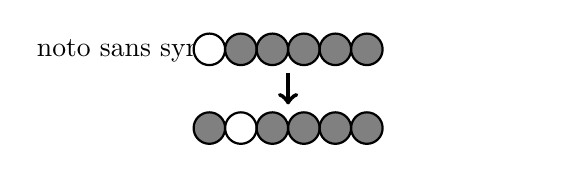
\begin{tikzpicture}
\node at (-0.6cm, 0) {\setmainfont{noto sans symbols 2}\normalsize☞};
\node at (2.6cm, 0) {\phantom{\setmainfont{noto sans symbols 2}\normalsize☜}};

\node[inner sep=0pt, minimum width=0.4cm, circle, draw, thick, fill=white] at (0,0) {};
\node[inner sep=0pt, minimum width=0.4cm, circle, draw, thick, fill=gray] at (0.4cm,0) {};
\node[inner sep=0pt, minimum width=0.4cm, circle, draw, thick, fill=gray] at (0.8cm,0) {};
\node[inner sep=0pt, minimum width=0.4cm, circle, draw, thick, fill=gray] at (1.2cm,0) {};
\node[inner sep=0pt, minimum width=0.4cm, circle, draw, thick, fill=gray] at (1.6cm,0) {};
\node[inner sep=0pt, minimum width=0.4cm, circle, draw, thick, fill=gray](a) at (2cm,0) {};

\draw[ultra thick, ->] (1cm, -0.3cm) -- (1cm, -0.7cm);

\node[inner sep=0pt, minimum width=0.4cm, circle, draw, thick, fill=gray] (b) at (0,-1.0cm) {};
\node[inner sep=0pt, minimum width=0.4cm, circle, draw, thick, fill=white] at (0.4cm,-1.0cm) {};
\node[inner sep=0pt, minimum width=0.4cm, circle, draw, thick, fill=gray] at (0.8cm,-1.0cm) {};
\node[inner sep=0pt, minimum width=0.4cm, circle, draw, thick, fill=gray] at (1.2cm,-1.0cm) {};
\node[inner sep=0pt, minimum width=0.4cm, circle, draw, thick, fill=gray] at (1.6cm,-1.0cm) {};
\node[inner sep=0pt, minimum width=0.4cm, circle, draw, thick, fill=gray] at (2cm,-1.0cm) {};

\end{tikzpicture}
\hfill
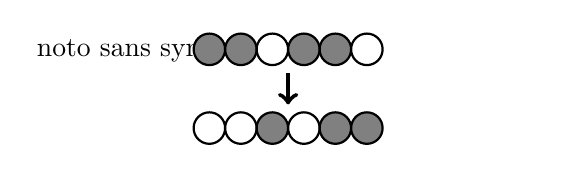
\begin{tikzpicture}
\node at (-0.6cm, 0) {\setmainfont{noto sans symbols 2}\normalsize☞};
\node at (2.6cm, 0) {\phantom{\setmainfont{noto sans symbols 2}\normalsize☜}};

\node[inner sep=0pt, minimum width=0.4cm, circle, draw, thick, fill=gray] at (0,0) {};
\node[inner sep=0pt, minimum width=0.4cm, circle, draw, thick, fill=gray] at (0.4cm,0) {};
\node[inner sep=0pt, minimum width=0.4cm, circle, draw, thick, fill=white] at (0.8cm,0) {};
\node[inner sep=0pt, minimum width=0.4cm, circle, draw, thick, fill=gray] at (1.2cm,0) {};
\node[inner sep=0pt, minimum width=0.4cm, circle, draw, thick, fill=gray] at (1.6cm,0) {};
\node[inner sep=0pt, minimum width=0.4cm, circle, draw, thick, fill=white](a) at (2cm,0) {};

\draw[ultra thick, ->] (1cm, -0.3cm) -- (1cm, -0.7cm);

\node[inner sep=0pt, minimum width=0.4cm, circle, draw, thick, fill=white] (b) at (0,-1.0cm) {};
\node[inner sep=0pt, minimum width=0.4cm, circle, draw, thick, fill=white] at (0.4cm,-1.0cm) {};
\node[inner sep=0pt, minimum width=0.4cm, circle, draw, thick, fill=gray] at (0.8cm,-1.0cm) {};
\node[inner sep=0pt, minimum width=0.4cm, circle, draw, thick, fill=white] at (1.2cm,-1.0cm) {};
\node[inner sep=0pt, minimum width=0.4cm, circle, draw, thick, fill=gray] at (1.6cm,-1.0cm) {};
\node[inner sep=0pt, minimum width=0.4cm, circle, draw, thick, fill=gray] at (2cm,-1.0cm) {};

\end{tikzpicture}
\end{center}

Similarly, if you touch the rightmost ball, all of the lights move one ball to the left. Then, if a light was ``pushed'' off the end, the two rightmost balls toggle on/off.

\begin{center}
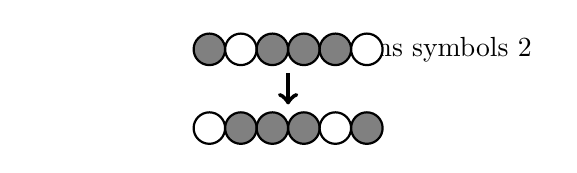
\begin{tikzpicture}
\node at (-0.6cm, 0) {\phantom{\setmainfont{noto sans symbols 2}\normalsize☞}};
\node at (2.6cm, 0) {\setmainfont{noto sans symbols 2}\normalsize☜};

\node[inner sep=0pt, minimum width=0.4cm, circle, draw, thick, fill=gray] at (0,0) {};
\node[inner sep=0pt, minimum width=0.4cm, circle, draw, thick, fill=white] at (0.4cm,0) {};
\node[inner sep=0pt, minimum width=0.4cm, circle, draw, thick, fill=gray] at (0.8cm,0) {};
\node[inner sep=0pt, minimum width=0.4cm, circle, draw, thick, fill=gray] at (1.2cm,0) {};
\node[inner sep=0pt, minimum width=0.4cm, circle, draw, thick, fill=gray] at (1.6cm,0) {};
\node[inner sep=0pt, minimum width=0.4cm, circle, draw, thick, fill=white](a) at (2cm,0) {};

\draw[ultra thick, ->] (1cm, -0.3cm) -- (1cm, -0.7cm);

\node[inner sep=0pt, minimum width=0.4cm, circle, draw, thick, fill=white] (b) at (0,-1.0cm) {};
\node[inner sep=0pt, minimum width=0.4cm, circle, draw, thick, fill=gray] at (0.4cm,-1.0cm) {};
\node[inner sep=0pt, minimum width=0.4cm, circle, draw, thick, fill=gray] at (0.8cm,-1.0cm) {};
\node[inner sep=0pt, minimum width=0.4cm, circle, draw, thick, fill=gray] at (1.2cm,-1.0cm) {};
\node[inner sep=0pt, minimum width=0.4cm, circle, draw, thick, fill=white] at (1.6cm,-1.0cm) {};
\node[inner sep=0pt, minimum width=0.4cm, circle, draw, thick, fill=gray] at (2.0cm,-1.0cm) {};

\end{tikzpicture}
\hfill
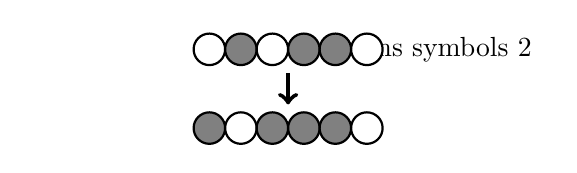
\begin{tikzpicture}
\node at (-0.6cm, 0) {\phantom{\setmainfont{noto sans symbols 2}\normalsize☞}};
\node at (2.6cm, 0) {\setmainfont{noto sans symbols 2}\normalsize☜};

\node[inner sep=0pt, minimum width=0.4cm, circle, draw, thick, fill=white] at (0,0) {};
\node[inner sep=0pt, minimum width=0.4cm, circle, draw, thick, fill=gray] at (0.4cm,0) {};
\node[inner sep=0pt, minimum width=0.4cm, circle, draw, thick, fill=white] at (0.8cm,0) {};
\node[inner sep=0pt, minimum width=0.4cm, circle, draw, thick, fill=gray] at (1.2cm,0) {};
\node[inner sep=0pt, minimum width=0.4cm, circle, draw, thick, fill=gray] at (1.6cm,0) {};
\node[inner sep=0pt, minimum width=0.4cm, circle, draw, thick, fill=white](a) at (2.0cm,0) {};

\draw[ultra thick, ->] (1cm, -0.3cm) -- (1cm, -0.7cm);

\node[inner sep=0pt, minimum width=0.4cm, circle, draw, thick, fill=gray] (b) at (0,-1.0cm) {};
\node[inner sep=0pt, minimum width=0.4cm, circle, draw, thick, fill=white] at (0.4cm,-1.0cm) {};
\node[inner sep=0pt, minimum width=0.4cm, circle, draw, thick, fill=gray] at (0.8cm,-1.0cm) {};
\node[inner sep=0pt, minimum width=0.4cm, circle, draw, thick, fill=gray] at (1.2cm,-1.0cm) {};
\node[inner sep=0pt, minimum width=0.4cm, circle, draw, thick, fill=gray] at (1.6cm,-1.0cm) {};
\node[inner sep=0pt, minimum width=0.4cm, circle, draw, thick, fill=white] at (2.0cm,-1.0cm) {};

\end{tikzpicture}
\end{center}

\newpage

\subsection*{Puzzle 2a: Unlock the Device}
Your player's main challenge in Act 2 is to figure out how to unlock the device by manipulating the device as follows:
\begin{center}
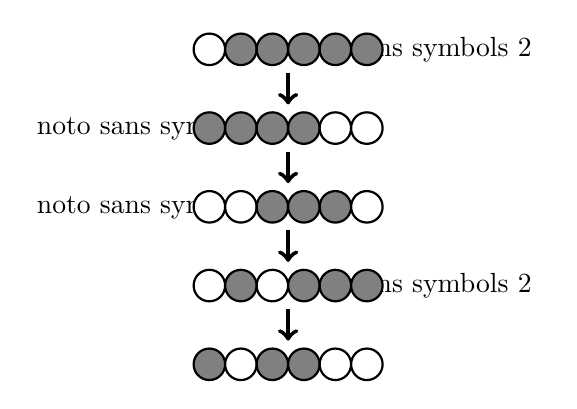
\begin{tikzpicture}
\node at (2.6cm, 0) {\setmainfont{noto sans symbols 2}\normalsize☜};

\node[inner sep=0pt, minimum width=0.4cm, circle, draw, thick, fill=white] at (0,0) {};
\node[inner sep=0pt, minimum width=0.4cm, circle, draw, thick, fill=gray] at (0.4cm,0) {};
\node[inner sep=0pt, minimum width=0.4cm, circle, draw, thick, fill=gray] at (0.8cm,0) {};
\node[inner sep=0pt, minimum width=0.4cm, circle, draw, thick, fill=gray] at (1.2cm,0) {};
\node[inner sep=0pt, minimum width=0.4cm, circle, draw, thick, fill=gray] at (1.6cm,0) {};
\node[inner sep=0pt, minimum width=0.4cm, circle, draw, thick, fill=gray](a) at (2cm,0) {};

\draw[ultra thick, ->] (1cm, -0.3cm) -- (1cm, -0.7cm);

\node at (-0.6cm, -1cm) {\setmainfont{noto sans symbols 2}\normalsize☞};

\node[inner sep=0pt, minimum width=0.4cm, circle, draw, thick, fill=gray] at (0,-1cm) {};
\node[inner sep=0pt, minimum width=0.4cm, circle, draw, thick, fill=gray] at (0.4cm,-1cm) {};
\node[inner sep=0pt, minimum width=0.4cm, circle, draw, thick, fill=gray] at (0.8cm,-1cm) {};
\node[inner sep=0pt, minimum width=0.4cm, circle, draw, thick, fill=gray] at (1.2cm,-1cm) {};
\node[inner sep=0pt, minimum width=0.4cm, circle, draw, thick, fill=white] at (1.6cm,-1cm) {};
\node[inner sep=0pt, minimum width=0.4cm, circle, draw, thick, fill=white](a) at (2cm,-1cm) {};

\draw[ultra thick, ->] (1cm, -1.3cm) -- (1cm, -1.7cm);

\node at (-0.6cm, -2cm) {\setmainfont{noto sans symbols 2}\normalsize☞};

\node[inner sep=0pt, minimum width=0.4cm, circle, draw, thick, fill=white] at (0,-2cm) {};
\node[inner sep=0pt, minimum width=0.4cm, circle, draw, thick, fill=white] at (0.4cm,-2cm) {};
\node[inner sep=0pt, minimum width=0.4cm, circle, draw, thick, fill=gray] at (0.8cm,-2cm) {};
\node[inner sep=0pt, minimum width=0.4cm, circle, draw, thick, fill=gray] at (1.2cm,-2cm) {};
\node[inner sep=0pt, minimum width=0.4cm, circle, draw, thick, fill=gray] at (1.6cm,-2cm) {};
\node[inner sep=0pt, minimum width=0.4cm, circle, draw, thick, fill=white](a) at (2cm,-2cm) {};

\draw[ultra thick, ->] (1cm, -2.3cm) -- (1cm, -2.7cm);

\node at (2.6cm, -3cm) {\setmainfont{noto sans symbols 2}\normalsize☜};


\node[inner sep=0pt, minimum width=0.4cm, circle, draw, thick, fill=white] at (0,-3cm) {};
\node[inner sep=0pt, minimum width=0.4cm, circle, draw, thick, fill=gray] at (0.4cm,-3cm) {};
\node[inner sep=0pt, minimum width=0.4cm, circle, draw, thick, fill=white] at (0.8cm,-3cm) {};
\node[inner sep=0pt, minimum width=0.4cm, circle, draw, thick, fill=gray] at (1.2cm,-3cm) {};
\node[inner sep=0pt, minimum width=0.4cm, circle, draw, thick, fill=gray] at (1.6cm,-3cm) {};
\node[inner sep=0pt, minimum width=0.4cm, circle, draw, thick, fill=gray](a) at (2cm,-3cm) {};

\draw[ultra thick, ->] (1cm, -3.3cm) -- (1cm, -3.7cm);

\node[inner sep=0pt, minimum width=0.4cm, circle, draw, thick, fill=gray] at (0,-4cm) {};
\node[inner sep=0pt, minimum width=0.4cm, circle, draw, thick, fill=white] at (0.4cm,-4cm) {};
\node[inner sep=0pt, minimum width=0.4cm, circle, draw, thick, fill=gray] at (0.8cm,-4cm) {};
\node[inner sep=0pt, minimum width=0.4cm, circle, draw, thick, fill=gray] at (1.2cm,-4cm) {};
\node[inner sep=0pt, minimum width=0.4cm, circle, draw, thick, fill=white] at (1.6cm,-4cm) {};
\node[inner sep=0pt, minimum width=0.4cm, circle, draw, thick, fill=white](a) at (2cm,-4cm) {};
\end{tikzpicture}
\end{center}

The clues that should suggest this solution to the player are hidden in the letter that they received from Uncle Elliot.

The patterns of X's and O's indicate the starting and ending patterns of lights and the first letters of each sentence describe the moves required to unlock the device.
\newpage

\section*{Act 3}
\textcolor{Red}{Describe what happens after unlocking the device by reading the following italicized text aloud.}

\textit{All six lights flash briefly and the force holding them together releases.}

\textit{``Well done!'' says a voice. You turn, and see your uncle standing next to the table in the middle of the room.}

\textit{On closer inspection, you realize that it isn't really your uncle, but rather some kind of hologram. Is this a recording?}

%\textit{If so, it must be quite old. Uncle Elliot appears to be several decades younger here than you remember him being.}
\textit{If so, it must be quite old. Uncle Elliot is much younger here than you remember.}

\textit{``If you're seeing this message,'' he says ``you must have unlocked the device. Now, it's time to use it and join me in the past.''}

\textit{Then, Uncle Elliot pauses dramatically for a moment before saying ``... and cut.''}

\newpage

\textit{The recording, however, keeps going.}

\textit{Your uncle moves over to the desk, on which a brown paper bag has appeared.}

\textit{He opens the bag and removes what looks like the receipt for an order from his favorite fast food restaurant.}

\textit{Then, he glances around the room, repeating the same pattern a few times: first to the southwest, then the southeast, then the northeast, and finally the east.}

\textit{``How delightful!'' he says, ``I can use my order to make a new safe combo.''}

\textit{As he bends over to examine the safe, he stops abruptly. ``Am I still recording? I certainly don't want this on tape.''}

\textit{Then, he freezes and the holograms all slowly fade away.}

\section*{Epilogue}
Test

%\input{aoa_components}
%
%\newpage
%
%\input{aoa_setup}
%
%\newpage
%
%\input{aoa_characters}
%
%\newpage
%
%\input{aoa_gameplay}
%
%\newpage
%
%\input{aoa_scoring}
%
%\vfill
%
%\hrulefill
%
%{\footnotesize \textbf{Design}: Michael Purcell \hfill \textbf{Contact}:~\href{mailto:mike@armiger.games}{mike@armiger.games}}
%
%%\begin{tabular}{ll}
%%\footnotesize{\doclicenseText} & \huge{\doclicenseIcon} \\
%%\end{tabular}
%
%\newpage
%
%\input{aoa_scoring_summary}

\end{document}
